\documentclass[pdf]{beamer}
\mode<presentation>

\usepackage[english]{babel}
\usepackage{amsmath,amssymb,listings}
\usepackage{graphicx}
\usepackage{xcolor}
\usepackage{pgfplots}

\usetikzlibrary{shapes.geometric}
\usetikzlibrary{shapes.misc}

\usetheme{Rochester}
\usecolortheme{beaver}
\useinnertheme{rounded}
\setbeamertemplate{navigation symbols}{} 

\begin{document}

\title{Transforming programs into \\ application specific processors}
\author{Arjan Boeijink \and Hendrik Folmer}
\institute{University of Twente}
\date{IFL 2017}

\frame{\titlepage}

%----------------------------------------------------------------------------------------
%	General introduction

\begin{frame}{The need for hardware specialisation}

\begin{block}{The current state of hardware world}
\begin{itemize}
\item All hardware is constrained by energy %(battery/electricity bill)
\item No more gains in clock frequency % (too much heat)
\item More parallelism is hard to find %and has diminishing returns
\item Alternative is specialisation % for energy efficient performance
\end{itemize}
\end{block}

\begin{block}{Customisable and reusable hardware with FPGAs}
\begin{itemize}
\item FPGAs are chips that can be 'rewired' to any hardware design
%\item Can contain 100s of multipliers and 10s MB of memory
\item Large size of current FPGAs allow for complex computations
%\item Avoiding the slow and expensive custom chip production
\item Slower than custom hardware but can be more specialized
\end{itemize}
\end{block}

\alert{Thus we have many programs to convert to efficient hardware}
\end{frame}


\begin{frame}{What makes hardware different from software?}
Hardware is a bounded box of computations with fixed in/outputs %, and internally it is a graph of smaller hardware components
\begin{center}
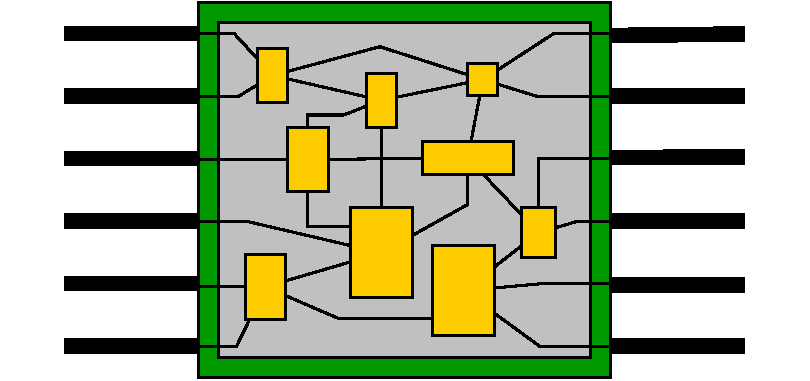
\includegraphics[scale=0.6]{schematic}
\end{center}

\begin{block}{Consequences for writing hardware as programs}
\begin{itemize}
\item No dynamic recursion or unbounded loops
\item All data is fixed size, no higher order functions
\item \alert{Too large means splitting in steps to reuse hardware over time}
\end{itemize}
\end{block}
\end{frame}

%----------------------------------------------------------------------------------------
%	Intro steps + BinGCD

\begin{frame}[fragile]{Binary GCD as program transformation example}
\framesubtitle{not obvious how to turn it into hardware}
%\begin{itemize}
%\item data dependent
%\item recursive
%\item function calls
%\end{itemize}
\begin{block}{}
\begin{verbatim}
binGCD :: Word32 -> Word32 -> Word32       
binGCD x 0 = x
binGCD x y = let
    a = dropTrailingZeros x
    b = dropTrailingZeros y
    (s,g) = (min a b, max a b)
  in binGCD s (g - s) <<< countTrZeros (x .|. y)

dropTrailingZeros :: Word32 -> Word32
dropTrailingZeros i = i >>> countTrZeros i

countTrZeros :: Word32 -> Word32
countTrZeros n = if odd n then 0 
  else countTrZeros (n >>> 1) + 1
\end{verbatim}
\end{block}

\end{frame}

\begin{frame}[fragile]{Flattening and desugaring the program}
\begin{columns}[T]
\column{.43\textwidth}
\begin{verbatim}
binGCD x y = if (y == 0)
 then x
 else
  let a = dropZeros x in
  let b = dropZeros y in
  let g = max a b in
  let s = min a b in
  let d = g - s in
  let r = binGCD s d in
  let o = x .|. y in
  let e = countZeros o in
  r <<< e
\end{verbatim}
\column{.57\textwidth}

\end{columns}

\end{frame}

%----------------------------------------------------------------------------------------
%	Step 2...

\begin{frame}[fragile]{Applying continuation passing style}
\begin{columns}[T] % the "c" option specifies center vertical alignment
\column{.43\textwidth} % column designated by a command
\begin{verbatim}
binGCD x y = if (y == 0)
 then x
 else
  let a = dropZeros x in
  let b = dropZeros y in
  let g = max a b in
  let s = min a b in
  let d = g - s in
  let r = binGCD s d in
  let o = x .|. y in
  let e = countZeros o in
  r <<< e
\end{verbatim}
\column{.57\textwidth}
\begin{verbatim}
binGCD x y k = if (y == 0)
 then cont x k
 else
  dropZeros x
   (\a -> dropZeros y
    (\b -> cont (max a b)
     (\g -> cont (min a b)
      (\s -> cont (g - s)
       (\d -> binGCD s d
        (\r -> cont (x .|. y)
         (\o -> countZeros o
          (\e -> cont (r <<< e) k)
   )))))))
\end{verbatim}
\end{columns}
\end{frame}

\begin{frame}[fragile]{Defunctionalising the continuations into data}
\begin{block}{Datatype for all continations}  %{datatype for continations each containing their free variables}
\begin{verbatim}
data Cont
  = CA Word32 Word32               Cont
  | CB Word32 Word32 Word32        Cont
  | CC Word32 Word32 Word32 Word32 Cont
  ....
\end{verbatim}
\end{block}

\begin{block}{}
\begin{small}
\begin{verbatim}

binGCD x y         k  = if (y == 0)
                   then cont x         k
                   else dropZeros x    (CA x y       k)
cont a (CA x y     k) = dropZeros y    (CB x y a     k)
cont b (CB x y a   k) = cont (max a b) (CC x y a b   k)
cont g (CC x y a b k) = cont (min a b) (CD x y a b g k)
\end{verbatim}
\end{small}
\end{block}

\end{frame}


\begin{frame}[fragile]{Using a stack instead of nested continuations}
\begin{small}
\begin{block}{using nested continuations}
\begin{verbatim}
binGCD x y          k  = if (y == 0)
                    then cont x         k
                    else dropZeros x    (CA x y        k)
cont a (CA x y      k) = dropZeros y    (CB x y a      k)
cont b (CB x y a    k) = cont (max a b) (CC x y a b    k)
cont g (CC x y a b  k) = cont (min a b) (CD x y a b g  k)
\end{verbatim}
\end{block}
\begin{block}{using a stack of flattened continuations}
\begin{verbatim}
binGCD x y         cs  = if (y == 0)
                    then cont x         cs
                    else dropZeros x    (CA x y      :cs)
cont a (CA x y    :cs) = dropZeros y    (CB x y a    :cs)
cont b (CB x y a  :cs) = cont (max a b) (CC x y a b  :cs)
cont g (CC x y a b:cs) = cont (min a b) (CD x y a b g:cs)
\end{verbatim}
\end{block}
\end{small}
\end{frame}


\begin{frame}[fragile]{From mutual recursion to a single step function}
\begin{block}{}
\begin{verbatim}
data Call = GCD Word32 Word32
          | DropZs Word32
          | CntZs Word32
		  | Cont Word32
\end{verbatim}
\end{block}
\begin{block}{}
\begin{verbatim}
step :: Call -> Stack -> (Call, Stack)
step (GCD x y)        cs = if y == 0
  then (Cont x      , cs             )
  else (DropZs x    , CA x y     : cs)
step (Cont a)        (CA x y     : cs) =
     (DropZs y      , CB x y a   : cs)
step (Cont b)        (CB x y a   : cs) =
     (Cont (max a b), CC x y a b : cs)
\end{verbatim}
%step (Cont g)        (CC x y a b   : cs) =
%     (Cont (min a b), CD x y a b g : cs)
\end{block}
\end{frame}


\begin{frame}{Hardware structure of the stack based state machine}
%\framesubtitle{with stack in a blockram it can be nice hardware, if the step function is not too large}
\hspace*{3em}
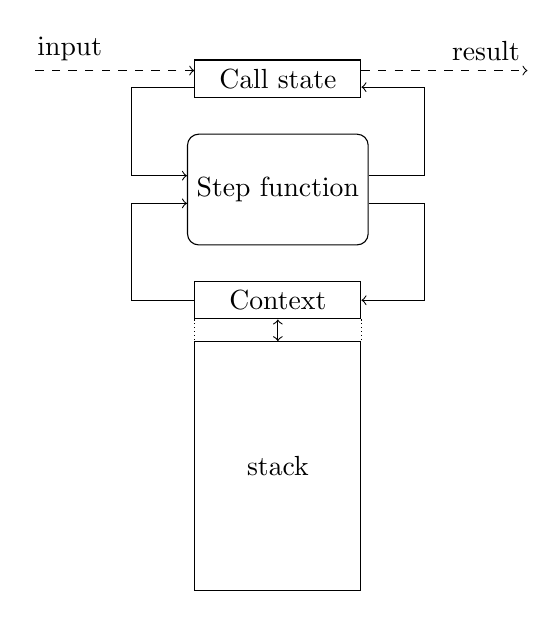
\begin{tikzpicture}
\node[draw, shape=rectangle, minimum width=6em] (st) {Call state};
\node[draw, shape=rectangle, minimum width=6em, minimum height=4em, below of=st, node distance=4em, rounded corners] (fun) {Step function};
\node[draw, shape=rectangle, minimum width=6em, below of=fun, node distance=4em] (con) {Context};
\node[draw, shape=rectangle, minimum width=6em, minimum height=9em, below of=con, node distance=6em] (ck) {stack};
\draw[densely dotted] (con.south west) -- (ck.north west);
\draw[densely dotted] (con.south east) -- (ck.north east);
\draw[->, dashed] ([yshift=0.3em]st.east) -- node[above, near end] {result} ([yshift=0.3em,xshift=6em]st.east);
\draw[<-, dashed] ([yshift=0.3em]st.west) -- node[above, near end] {input} ([yshift=0.3em,xshift=-6em]st.west);
\draw[->] ([yshift=0.5em]fun.east) -| ([xshift=2em]fun.north east) |- ([yshift=-0.3em]st.east);
\draw[->] ([yshift=-0.3em]st.west) -| ([xshift=-2em]fun.north west) |- ([yshift=0.5em]fun.west);
\draw[->] ([yshift=-0.5em]fun.east) -| ([xshift=2em]fun.south east) |- (con.east);
\draw[->] (con.west) -| ([xshift=-2em]fun.south west) |- ([yshift=-0.5em]fun.west);
\draw[<->] (con.south) -- (ck.north);
\end{tikzpicture}
\end{frame}

\begin{frame}[fragile]{Splitting off the data stack}
\begin{block}{}
\begin{verbatim}
step :: Call -> Stack -> (Call, Stack)
step (Cont a)       (CA x y      :cs) =
     (DropZs y,      CB x y a    :cs)
step (Cont b)       (CB x y a    :cs) =
     (Cont (max a b),CC x y a b  :cs)
step (Cont g)       (CC x y a b  :cs) =
     (Cont (min a b),CD x y a b g:cs)
\end{verbatim}
\end{block}
\begin{block}{}
\begin{verbatim}
step :: State -> CtrlStack -> DataStack ->
       (State ,  CtrlStack ,  DataStack)
step Cont    (CA:cs)       (a:y:x:ds) = 
    (DropZs,  CB:cs,      y:a:y:x:ds)
step Cont    (CB:cs)     (b:a:y:x:ds) = 
    (Cont,    CC:cs,    g:b:a:y:x:ds) where g=max a b
step Cont    (CC:cs)   (g:b:a:y:x:ds) = 
    (Cont,    CD:cs,  s:g:b:a:y:x:ds) where s=min a b
\end{verbatim}
\end{block}
\end{frame}

\begin{frame}[fragile]{Optimizing the control}
\begin{block}{}
\begin{small}
\begin{verbatim}
data Label = BinGCD | T1 | E1 | CA | CB | CC | ...
type CtrlFun = Bool->Label->CtrlStack->(Label,CtrlStack)
\end{verbatim}
\end{small}
\end{block}

\begin{block}{}
\begin{verbatim}
step :: Label -> DataStack -> (CtrlFun,DataStack)
step BinGCD        (y:x:ds) =
  (branch E1 z,     y:x:ds) where z = y == 0
step T1            (y:x:ds) = 
  (ret        ,       x:ds)
step E1            (y:x:ds) = 
  (call DropZs,   x:y:x:ds)
step CA          (a:y:x:ds) = 
  (call DropZs, y:a:y:x:ds)
step CB        (b:a:y:x:ds) = 
  (next     , g:b:a:y:x:ds) where g = max a b
\end{verbatim}
\end{block}

\end{frame}


\begin{frame}[fragile]{Splitting into components}
\begin{block}{}
\begin{verbatim}
step :: Label -> DataStack -> (CtrlFun,DataStack)
step CA          (a:y:x:ds) = 
  (call DropZs, y:a:y:x:ds)
\end{verbatim}
\end{block}

\begin{block}{}
\begin{verbatim}
step :: Label -> (CtrlFun,Input,Input,AluOp,StackMod)
step GCD = (branch E1  ,peek 0,lit 0 , isEq ,keep)
step T1  = (ret        ,peek 1,lit 0 , pass ,popNPush 2)
step E1  = (call DropZs,peek 1,lit 0 , pass ,push)
step CA  = (call DropZs,peek 1,lit 0 , pass ,push)
step CB  = (next       ,peek 1,peek 0, max  ,push)
\end{verbatim}

\begin{verbatim}type Input = DataStack -> Word32
type AluOp = Word32 -> Word32 -> Word32
type StackMod = Word32 -> DataStack -> DataStack
\end{verbatim}
\end{block}
\end{frame}

\begin{frame}[fragile]{Using microcode to control each component}
\begin{block}{}
\begin{verbatim}
microcode :: Label -> (Ctrl,Input,Input,AluOp,StAction)
microcode pc = case pc of
  BinGCD -> (Branch E1  , S 0, I 0, IsEq , Keep)
  T1     -> (Return     , S 1, I 0, Pass , PopNPush 2)
  E1     -> (Call DropZs, S 1, I 0, Pass , Push)
  CA     -> (Call DropZs, S 1, I 0, Pass , Push)
  CB     -> (Next       , S 1, S 0, Max  , Push)
  CC     -> (Next       , S 2, S 1, Min  , Push)
\end{verbatim}
\end{block}

\begin{block}{}
\begin{verbatim}
data AluOp = Pass | Add | Sub | Or | Min | ...

alu :: AluOp -> Word32 -> Word32 -> Word32
alu Pass  x _ = x
alu Add   x y = x + y
alu Sub   x y = x - y
\end{verbatim}
\end{block}

\end{frame}


\begin{frame}{Overview of resulting hardware architecture}
\hspace*{2em}
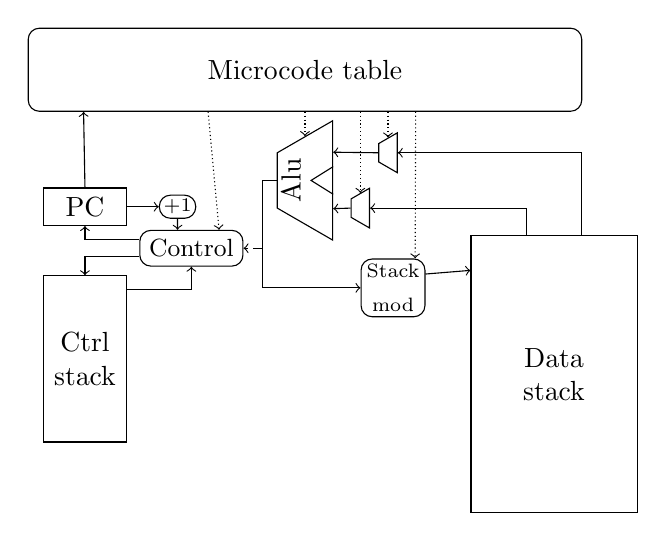
\begin{tikzpicture}
%\node[draw, shape=rectangle, minimum width=6em, minimum height=8em] (im) {InstrMem};
\node[draw, shape=rectangle, rounded corners, minimum width=20em, minimum height=3em] (mc) {Microcode table};
%\node[draw, shape=rectangle, rounded corners, minimum width=8em, right of=mc, xshift=1em] (dec) {Decode};
\node[draw, shape=rectangle, minimum width=3em, below left of=mc, node distance=7em, xshift=-3em] (pc) {PC};
\node[draw, shape=rectangle, rounded corners, right of=pc, xshift=0.5em, inner sep=0.15em] (npc) {\begin{scriptsize}$+1$\end{scriptsize}};
\node[draw, shape=rectangle, rounded corners, right of=pc, xshift=1em, yshift=-1.5em] (cc) {\begin{small}Control\end{small}};
\node[draw, shape=rectangle, minimum width=3em, minimum height=6em, below of=pc, node distance=5.5em, align=center] (cs) {Ctrl\\stack};
\node[draw, shape=rectangle, minimum width=6em, minimum height=10em, below of=mc, node distance=10em, align=center, xshift=9em, yshift=-1em] (ds) {Data\\stack};
\node[draw, shape=trapezium, minimum width=3em, minimum height=2em, below of=mc, node distance=4em, xshift=0em, rotate=90] (alu) {};
\node[xshift=-0.5em, rotate=90] at (alu.center) {Alu};
\node[draw, shape=rectangle, rounded corners, below right of=alu, node distance=4.5em, yshift=-0.7em, inner sep=0.2em, align=center] (sp) {\begin{scriptsize}Stack\end{scriptsize}\\\begin{scriptsize}mod\end{scriptsize}};
\draw ([yshift=0.5em] alu.south) -- ([xshift=-0.8em] alu.south) -- ([yshift=-0.5em] alu.south);
\node[draw, shape=trapezium, minimum width=1em, minimum height=0.5em, right of=alu, node distance=3em, yshift=1em, rotate=90] (ina) {};
\node[draw, shape=trapezium, minimum width=1em, minimum height=0.5em, right of=alu, node distance=2em, yshift=-1em, rotate=90] (inb) {};
\draw[->] (ina.north) -- (alu.south east);
\draw[->] (inb.north) -- (alu.south west);
\draw[->] ([xshift=1em] ds.north) |- (ina.south);
\draw[->] ([xshift=-1em] ds.north) |- (inb.south);
\draw[->] (pc.north) -- ([xshift=-8em] mc.south);
\draw[->] (pc.east) -- (npc.west);
\draw[->] (npc.south) -- ([xshift=-0.5em] cc.north);
%\draw[->] ([yshift=1.85em] im.east) -- (dec.west);
\draw[->] ([yshift=0.3em] cc.west) -| (pc.south);
\draw[->] ([yshift=-0.3em] cc.west) -| (cs.north);
\draw[->] ([yshift=2.5em]cs.east) -| (cc.south);
\draw[->] ([yshift=0.5em] sp.east) -- ([yshift=3.75em] ds.west);
\draw[->] (alu.north) -- ([xshift=-0.5em] alu.north) |- (sp.west);
\draw[->, densely dashed] (alu.north) -- ([xshift=-0.5em] alu.north) |- (cc.east);
\draw[->, densely dotted] ([xshift=-3.5em] mc.south) -- ([xshift=1em] cc.north);
\draw[->, densely dotted] ([xshift=0em] mc.south) -- (alu.east);
\draw[->, densely dotted] ([xshift=2em] mc.south) -- (inb.east);
\draw[->, densely dotted] ([xshift=3em] mc.south) -- (ina.east);
\draw[->, densely dotted] ([xshift=4em] mc.south) -- ([xshift=0.8em]sp.north);
\end{tikzpicture}
\end{frame}


\begin{frame}{From program to 'processor' in just 10 transformation steps}
\framesubtitle{using only basic hardware principles and well known transformations}
%conclusion on steps taken\\developers knowledge in first step (cps sequentialize step size determination)
\begin{block}{}
\begin{enumerate}
 \item Desugaring of the program
 \item Choosing step size and applying the CPS transformation
 \item Defunctionalisation of the continuations
 \item Introducing a stack for continuations
% \item Splitting the program in instruction sized parts
%  \item key choices to make, simple iterative process (potential long)
 \item Stepwise execution by merging all mutual recursive functions
%  \item fully automated process if Ingmar's research succeeds
 \item Separating the data stack for local values
%  \item determined by programming language and hardware constraints
 \item Refactor to a control stack with a program counter
%  \item just a minor simplification and optimization
 \item Division into simple orthogonal components
%  \item straightforward process with many choices, but all minor

 \item Control by a table of horizontal microcode
%  \item this refactoring step could be automated
% \item Create an instruction set as microcode compression
%  \item just a pattern finding puzzle with many minor details
 \item Making the hardware description synthesizable
% \item Final step bonus step: introduce pipelining?
\end{enumerate}
\end{block}

%\begin{block}{Differences with a 'real' processors}
%\end{block}

\end{frame}


\begin{frame}{Part 2: applying the transformation process}

\begin{block}{A functional hardware design process}
\begin{enumerate}
\item Write algorithm as executable Haskell code
\item Convert all data to fixed size
\item Try avoid using expensive constructs %(floating point, etc.)
\item Analyse hardware resource requirements
\item Make area/time tradeoff to fit target platform
\item Write control/glue logic for computation over time
\end{enumerate}
\end{block}

\begin{block}{Using Clash as hardware description language}
\begin{itemize}
\item Subset of Haskell that can be compiled to hardware
\item A Clash program describes the structure of the hardware
\item Can use most high level FP abstractions % for higher level code
\item Fixed size datatypes with type level numerals
\end{itemize}
\end{block}

\end{frame}

%----------------------------------------------------------------------------------------
%	Seqlogic intro

\begin{frame}{The crucial choice of what to compute each single cycle}

%$execution~time~=~number~of~steps~*~cycle~time$

\begin{block}{Performance and hardware cost from explicit steps}
\begin{itemize}
\item Placing cycle boundaries $~=>~$ number of steps
\item The slowest step $~=>~$ clock frequency
\item More work in a step $~=>~$ more parallel hardware
\item Ordering of steps $~=>~$  memory requirements
\item Similar steps in program $~=>~$ hardware reuse
\end{itemize}
\end{block}

\begin{block}{The problem and solution match up}
\begin{itemize}
\item Manual writing control code is too much work
\item The only choice in transformation process is where to CPS
\item Making area/time tradeoffs is the essence of hardware design
%\item Also want to keep hardware design process incremental
\end{itemize}
\end{block}

%why seqlogic? give developers a way of designing/specifying functionality and clock boundaries\\
%first step : CPS??

\end{frame}

%----------------------------------------------------------------------------------------
%	Seqlogic 

\begin{frame}[fragile]{The sequential logic monad with explict clock cycles}
\framesubtitle{used both for simulation and hardware generation}
\begin{block}{}
\begin{verbatim}
normalize :: Vector n SFixed32 -> 
  SeqLogic s i o (Vector n SFixed32)
normalize xs = do
   let sqs = xs .*. xs
   clock
   let n = sumV sqs
   clock
   let invsq = fast_invSqrt n
   clock
   return (invsq *. xs)
\end{verbatim}
\end{block}

\begin{block}{}
\begin{verbatim}
n *. xs = zipWithV (*) (replicateI n) xs
xs .*. ys = zipWithV (*) xs ys
sumV xs = treeFoldV (+) xs
fast_invSqrt n = ...
\end{verbatim}
\end{block}

\end{frame}

%----------------------------------------------------------------------------------------
%	Seqlogic threads

\begin{frame}[fragile]{Concurrent execution as coprocessors in hardware}
\begin{block}{Problem: keep hardware busy when doing a slow computation}
Interleaving multiple computation cycle by cycle is a mess \\
Solution: fork off slow computation as seperate 'thread'
\end{block}

\begin{block}{}
\begin{small}
\begin{verbatim}
  divider <- start (divide x y)
  clock
  ...
  
  ...
  clock
  d <- finish divider
  ...

divide :: Number -> Number -> SeqLogic s i o Number
divide x y = do
  let divisor = abs y
  ...
\end{verbatim}
\end{small}
\end{block}

\end{frame}

\begin{frame}[fragile]{Simulation and transforming the SeqLogic monad}
\begin{block}{Cycle accurate simulation of SeqLogic}
Every cycle execute statements one by one till a $clock$ or blocking \\
Can be simulated together with other Clash code:
\begin{verbatim}
interpretSeqLogic :: (forall s. SeqLogic s i o ())
  -> Signal (Maybe i) -> Signal (Maybe o)
\end{verbatim}
\end{block}

\begin{block}{prog2proc: a tool for generating specialised processors}
\begin{itemize}
\item Source (SeqLogic) to source (Clash) tranformation
\item Using haskell-src-exts parser to extract the code
\item Finding the type of every variable to group them
\item Analyse livetimes of variables for memory allocation
\item Count number of inputs/outputs/ports for ALU and memory
\item Generate microcode table controlling all components
\end{itemize}
\end{block}

\end{frame}

\begin{frame}{Summary}
%\framesubtitle{a processor is a thing that executes programs in many bounded steps}

\begin{itemize}
\item Specialisation of hardware is required for improving efficiency
\item Going from program to processor uses well known transformations
\item Reusing hardware over time yields a processor like architecture
\item Cycle boundaries are the key choice in hardware design
\item The rest of the transformations are easily automated
\item A sequential EDSL for Haskell based hardware design process
%\item Five times less control code than manual hardware description
\end{itemize}

\alert{Why waste time on compilers for 'unprogrammable' hardware \\ if you can just generate hardware instead?}

\end{frame}


\begin{frame}{Future work}

\begin{block}{Exploring the relation between software and hardware}
\begin{itemize}
\item Start from language semantics instead of specific programs
\item Can we calculate compilers and processors from semantics?
\item Extend transfromations for other language features %(memory/complex control flow)
\item Identify software equivalents for hardware optimisations
\end{itemize}
\end{block}

\begin{block}{Improving the transformation tool}
\begin{itemize}
\item Clash plugin instead of source to source rewriting
\item Software pipelining and data parallelism support
\item Higher level abstractions for space-time tradeoffs
% Automating parts of the process or better refactoring tools\\
%Work out the process for pipelining and data parallelism?
\end{itemize}
\end{block}

\end{frame}

\begin{frame}
\Huge{\centerline{Questions?}}
%question for audience: how to combine explicit execution steps with higher level FP abstractions
\end{frame}

\begin{frame}{Practical testcase: the iterative closest point algorithm}
\begin{block}{Matching scan points from a laser range finder}
for each point find 2 closest points in other scan \\
build system of equations using normal vectors \\ 
solve the system using QR decomposition
\end{block}

\begin{block}{Our experience with using the EDSL}
Five times less control code than manual hardware description \\
Sequentialising incrementally saves a lot of debugging \\
missing segmented vectors and software pipelining
\end{block}

\end{frame}


\begin{frame}[fragile]{The most complex part of our ICP code}
% icp example -> vectorizing \\ clash?
\begin{block}{}
\begin{verbatim}
gram_schmidt :: Ref s Mat4xn -> 
  SeqLogic s i o (Ref s Mat4xn)
gram_schmidt v = do
  u <- allocArr d4
  loop 0 upto 3 $ \j -> do
     v_j <- peek (v?j)
     t <- loopAccum (0, upto, j-1) v_j $ \k t -> do
        u_k <- peek (u?k)
        vj_uk <- inline $ v_j `project` u_k
        clock
        return (t .-. vj_uk)
     u?j <~< inline $ normalize t
return u
\end{verbatim}
\end{block}

\begin{block}{}
Using inline functions, zero overhead loops and explicit memory
\end{block}

\end{frame}

\begin{frame}[fragile]{Another piece of the ICP code}
\begin{scriptsize}
\begin{verbatim}
  loop 0 upto (180-1) $ \i -> do
    let pointX = vecPx!!i
    let vecDx = pointX -. vecQx
    clock
    let pointY = vecPy!!i
    let vecDy = pointY -. vecQy
    clock
    vecMagSq <- vecDx.*.vecDx |^(.+.)^| vecDy.*.vecDy
    clock
    let (j,k) = indexSmallestTwo vecMagSq
    normLV <- start normLineVec
    clock
    let px  = vecPx!!i
    let mxA = vecQx!!j
    let mxB = vecQx!!k
    inject normLV (px, mxA, mxB)
    vecMx?i <~ mxA
    clock
    let py  = vecPy!!i
    let myA = vecQy!!j
    let myB = vecQy!!k
    inject normLV (py, myA, myB)
    vecMy?i <~ myA
    clock
    vecNx?i <~< extract normLV
    clock
    vecNy?i <~< finish normLV
\end{verbatim}
\end{scriptsize}


\end{frame}


\end{document}
